\section{第二原则：不完备性原则}

意义需要持续的投入才能不退回噪声，而投入总要有方向。方向的问题看起来很技术：给它一个目标函数，系统就能在上面搜索。但目标函数不是从天上落下来的，它是被写进去的，而写进去就意味着做过一次压缩。第二原则处理的正是这次压缩：把多维的价值压成可优化的目标，会损失什么，损失的这部分能不能被补回来，以及补回来的东西只能从哪里来。

\subsection{价值对齐中的标量化与取舍}

先看压缩本身。一个优化问题的目标是让一个标量函数取到最大或最小，而人的价值判断从来不是一个标量。正义、美、信任、安全、公平，这些东西内部有多个维度，维度之间不能彼此换算，而且同一个词在不同语境里指向不同的内容。把它们写成一个数，需要事先确定各维的权重；权重一旦确定，争议就不再出现在优化过程里，而是被藏进了参数。于是出现一个结构性的结果：优化做得越好，被藏起来的那部分分歧显得越少，而它并没有消失。

\subhead{标量化的取舍}

把多个评价维度写成一个目标，必须规定它们如何比较。加权求和是常用做法。设$v_j(\mathbf x)$为方案$\mathbf x$在第$j$个维度上的归一化评价，$w_j$为相应权重，
\begin{equation}
U(\mathbf x)=\sum_{j=1}^{m}w_jv_j(\mathbf x),\qquad w_j\ge0,\quad \sum_{j=1}^{m}w_j=1
\end{equation}
$U$是综合评价，$m$是维度数。归一化确定比较刻度，权重确定允许怎样的补偿。当$m>1$时，同一个综合得分通常对应多组维度组合；只保留$U$，便不能恢复原来的全部评价。安全下降多少可以由效率增加补偿，已经写在权重和函数形式中。

这一步使问题可以优化，也使一部分分歧移到了建模之前。相同的方案可能在不同权重下交换次序，某项指标被赋予零权重时，它的变化不再影响总分。需要检查的是评价是否保留了决定所必需的差异，以及被舍去的差异有没有其他表达和救济的通道。高维空间的几何现象不能替这项检查作出结论，具体取舍必须落到被采用的目标上。

\subhead{聚合的不可能性}

多个主体的偏好需要另一组判据。Arrow定理讨论三个或以上备选方案、允许任意个人偏好排序的情形，表明满足帕累托一致与无关选项独立性的社会排序规则必然具有独裁性。\cite{arrow1951social} Gibbard与Satterthwaite则说明，在相应的无约束偏好域、至少三个可能获选结果和确定性投票规则下，策略不可操纵与非独裁不能同时满足。\cite{gibbard1973manipulation,satterthwaite1975strategy} 这些定理定位了聚合条件之间的冲突。采用何种偏好域、信息和程序，仍是制度设计的选择。

固定权重的加权和还会限制可选解。在一般非凸多目标问题中，改变正权重只能取得受支撑的帕累托解，某些非凸前沿上的有效解始终取不到。\cite{das1997closer} 决策者选择了加权和，也就选择了一种候选筛选方式。保留原始指标、约束与其他标量化方法，才能检查哪些取舍被这种方式排除。

\subhead{优化器携带的先验}

优化器的效果还取决于任务分布。无免费午餐结果在有限搜索空间、对全部目标函数按规定方式平均等条件下成立：算法在某类问题上的优势，需要由该类问题的结构来解释。\cite{wolpert1997no} 实际训练和部署面对的是特定数据与任务，目标、表示和采样由此携带先验。考察这些先验，有助于说明一个代理指标为何在训练环境有效，换到另一种场景却偏离要求。

\subhead{代理指标成为目标之后}

代理指标被当成目标之后会发生什么，有一批记录得很清楚的例子。一个被训练去得分的赛艇智能体发现，原地打转反复穿过得分点比完成赛道更快，于是它不去比赛；这是 2016 年公开记录的真实案例，训练目标没有写错，被写下来的那个指标与真正想要的东西之间本来就有一道缝。\cite{amodei2016concrete} 类似的机制在制度层面同样成立：用代码行数衡量生产率会鼓励冗余，用论文数量衡量学术产出会鼓励把一项研究切碎成若干最小可发表单元，用等待时间衡量医院效率会把等待转移到没有计入的地点。这类现象通常被概括为一句话：指标一旦成为目标就不再是好指标。\cite{goodhart1975problems}\cite{strathern1997audit} 它的机制并不神秘，就是压缩后剩下的那些维度里包含了一个便宜的替代路径，优化过程就可能利用这条路径。

把评比压成分数之后发生的位移，有两个记录得比较完整的例子。美国的量刑指南在 1987 年生效时，试图用一套评分表把量刑从法官的自由裁量转为可以计算的规则，犯罪等级与犯罪历史各占一项，总分对应刑期区间；它的初衷是减少地区差异与歧视，而随后的研究普遍指出裁量没有消失，它从法官的判决环节转移到了检察官的指控环节和指南的修订环节，2005 年联邦最高法院在布克案中判定该指南只具有参考性。\cite{us2005booker} 卫生系统提供了方向相同的另一个例子：为了达成四小时内接诊的等待时间指标，病人在进入急诊科之前的等待被转移到救护车上，指标随之达标，而病人的总等待时间没有改善。 这类位移反复出现，原因不是执行者不诚实，而是被计量的那一段与真正被关心的那一段不是同一段。

\subhead{压缩本身不是问题}

工程安全系数、临床阈值和法律构成要件，都把复杂情况转成可操作的判据。判据的质量，要看它保留了哪些关键差异，以及错误出现后能否被发现和纠正。公开依据、保留申诉、复核结果并更新标准，使被折价的维度仍有机会重新进入决定。\cite{ashby1956cybernetics}

标准需要修订，修订也需要依据。形式证明、经验校准和公共授权分别提供不同的依据。逻辑学能够说明第一类依据的某些边界，后两类则要考察对象反馈、参与程序与责任。

\subsection{哥德尔缝隙的填充}

哥德尔在 1931 年证明了两件事，两个定理的表述必须准确。第一不完备性定理：任何一个一致的、公理集可有效枚举的、并且强到足以表达基本算术的形式系统，都存在一个命题，该命题及其否定都不能在系统内被证明。第二不完备性定理：这样一个系统如果是一致的，它不能在自身内部证明自己的一致性。\cite{godel1931} 图灵在 1936 年给出了计算版本的对应结果：不存在一个通用程序能判定任意程序是否会在有限步内停机。\cite{turing1936} 更晚的算法信息论把这件事推得更细，一个形式系统能够证明的停机命题，其复杂度受系统自身复杂度的上界约束。\cite{chaitin1987}

\subhead{形式证明的对象}

这些定理约束满足相应条件的形式系统与通用判定程序。神经网络通过数据和优化形成参数，推理时的行为不能直接等同于一套固定公理的演绎。人的数学判断也没有现成的一致性证明。Lucas与Penrose围绕心智和形式系统提出过不同论证，\cite{lucas1961minds,penrose1989emperor} 这些讨论需要分别检查其关于人和机器的假设。

\subhead{本书引用它的方式}

Tarski关于真理的结果进一步区分了对象语言与元语言：足够强的算术语言，不能在自身内部定义满足通常要求的完整真理谓词。\cite{tarski1936wahrheitsbegriff} 工程验证则区分实现与规范。微内核的形式化验证可以严格检查实现是否符合所建模的规范，\cite{klein2009sel4} 规范是否表达了使用者的要求，还要通过需求分析、测试和审查判断。这是两种不同的论证关系，规范的正当性不能由实现正确性替代。

这类边界在工程上有一个通用的名称：信任根。任何验证链条都必须停在一个未被验证的起点上，而把这个起点选在哪里是一个工程决定。微内核的形式验证之所以有说服力，部分原因是它把信任根缩得很小，硬件、汇编层、编译器与启动代码仍在被信任的范围内，但它们被明确列出，可以被单独审查，而不是混在整条链里不被提及。把假设写在明处不会让系统变得绝对可靠，它只是让可靠性依赖什么变得可以被追问。

\subhead{莱斯定理与工具的取舍}

Rice定理讨论图灵可计算的部分函数：任何非平凡的外延语义性质，都不存在对任意程序总能终止且正确判定的通用算法。\cite{rice1953classes} 全部程序上的完备判定因此受到限制。静态分析可以限制语言与程序类别，或在一般情形中选择可靠近似、接受误报或漏报；运行时检查与人工复核再承担其他部分。具体工具的能力，要按所覆盖的程序范围评价。

这个取舍写成两个集合之间的关系就是，

\begin{equation}
B\subseteq L\quad(\text{不漏报}),\qquad L\subseteq B\quad(\text{不误报})
\end{equation}

$B$为具有目标语义性质的程序集合，$L$为工具报告的集合。$B\subseteq L$表示不漏报，$L\subseteq B$表示不误报。对任意程序均终止的工具，若对Rice定理所述的非平凡外延性质同时满足两式，就构成不存在的通用判定器。限制程序类别后可以同时做到两者，因而工具说明必须列出覆盖范围。集合关系本身只规定可靠性与完备性，具体任务还要比较各类错误的后果。

\subhead{依据、授权与责任}

形式结论依赖公理与规则，经验结论依赖对象与观测，行动决定还依赖权利与授权。\key{优化可以按既定标准搜索，采用标准的理由仍须被提出和审查。} 模型可以生成标准，也可以检查一致性；决定哪些损失可接受、谁有权承担风险，需要让受影响者进入相应程序。后者的理由来自人的权利、利益和责任关系。

\subhead{这条结论的边界}

标准的修订可以来自新观测、形式推导、反例和公开争议。谁提出、谁审核、谁作出决定，应当留下可追溯的记录；承担风险的人需要了解依据，并有质疑与救济的通道。证据可以提高决定的可靠性，授权程序则处理决定者与承受者之间的关系。

通用不可判定与具体问题的进展同时存在。忙碌海狸函数没有通用可计算上界，具体的小规模情形仍能被证明；2024年的协作项目确认了五状态情形的取值47176870。\cite{bbchallenge2024} 自动搜索与形式化工具在这里扩大了能够确认的范围。知识形成既需要发现候选，也需要查明具体证明依赖什么。

缺口必须由外部填，而外部并不是一片均匀的空间，它有结构：有些位置承担的是可被检验的判断，有些位置只是把判断转手。真正能够提供判据的位置，必须同时具备条件与代价：它需要持续投入才能维持，它需要外部参照才能标定，它的错误必须落在自己身上。这些条件把问题从“谁更聪明”转到“谁站在哪里”，也把讨论带到下一节：价值正在向哪些位置沉淀，以及为什么是那些位置。

\subsection{高黏滞沉淀区：价值向不可低成本伪造处移动}

\subhead{流向，而不是清单}

前面留下的问题是：这些不能被低成本伪造的功能，具体落在什么位置上。回答这个问题要换一个问法，不问哪些工作有价值，而问技术会优先改造什么、留下什么。技术流向低黏滞区，这是一个近乎机械的规律。资本的流向由投入产出比决定，而投入产出比与技术能降低多少成本直接相关。一个环节如果可以被表示为规则、编码为流程、量化为指标，它被改造的速度就快；一个环节如果依赖具体的人、具体的时间、具体的身体，它被改造的速度就慢。这不是价值判断，只是资源配置的结果。

由此可以提出一条待观察的流向：当常规产出便宜，某些难以供应的互补功能会变得相对重要。它们能否获得高报酬和稳定位置，还取决于需求、预算、产权与议价。高黏滞本身也可能意味着改造机会，不能直接作为职业前景的保证。

\subhead{高黏滞位置的判据}

一个位置能否成为高黏滞沉淀区，可以用三个条件来判定，它们分别对应投入端的资源势垒、过程的时间刚性和系统结构上的耦合程度。条件之一与投入有关：这个位置上的工作是否要求不可替代的投入，一段无法跳过的时间、一个必须亲历的过程、一次不能转嫁的消耗。外科医生的手需要多年训练才能形成，心理咨询师的判断需要在大量真实个案中积累，飞行员在紧急情况下的处置依赖于模拟机和真实飞行的小时数。这些投入的特征是它们不能被购买，只能被经历，因此一个人的技能水平和他的时间投入之间存在无法绕开的关系。

条件之二是时间刚性：这个位置上的过程是否有内禀的时间尺度，压缩它会改变结果。作物有生长周期，伤口有愈合周期，人有学习曲线，组织有信任积累的速率。这些周期不因为信息处理变快而变短。这个条件比第一个更强，因为它给出了一条筛选线：一个允许被无限加速的工作，最终会被加速掉；一个依赖慢变量的工作，会保留下来。两个条件的区别在于，第一个条件随着技术能力提高可能被削弱：如果某一天训练可以被打包植入，不可替代的投入就不成立了；第二个条件不会，因为它来自物理过程本身的时间尺度。

条件之三是拓扑耦合：这个位置是否嵌在一个需要现场判断的复杂系统中。电网调度员、重症监护医生、事故现场指挥、飞机机长、法官，这些角色的共同点不是技能高超，而是他们处在一个信息不完整、后果不可逆、需要在有限时间内做出不可撤回决定的节点上。这种位置无法被拆解成流程，因为它的核心功能就是在流程失效时做出判断。三个条件同时成立的位置，构成了沉淀区的候选集合。

\subhead{几个确定的沉淀区}

把这个判据用上去，可以看到几类位置会持续吸收价值，而它们各自的理由并不相同。验证与信任是其中最清楚的一类，理由是当生成变得便宜，确认变得昂贵，检验和认证的功能就获得了系统性的溢价。这里的位置不限于技术验证，也包括人与人之间的信任中介：推荐、担保、背书、声誉评价。一个可以被追溯的判断记录，是这种中介的基础材料，而它的积累速度受制于人类兑现承诺的速度，于是这一类位置天然是慢的。

照护与陪伴对应另一种条件：合适技能、时间、连续性，以及某些关系中的特定在场。工具与组织可以改善服务，需求增长却不会自动兑现为工资上涨。公共支付、家庭资源、劳动制度与议价，会决定成本落在哪里。

判断与裁决处理证据、风险、利益和权利。计算可以改进估计和比较，合法采用标准仍需相应授权、职责与程序。直接承受者、专业者和公共代表各有不同位置，制度要让这些位置能够交流、制衡与追责。

教育中的长期塑造是第五类，也是最容易被低估的一类。它包含了知识传递，但核心不在此。一个人从孩子长成成年人，其中有十几年的时间，他的判断、品味、注意力和对自己能力的认知都在被周围的人塑造。这个过程无法被外包，因为它依赖的是长期的关系和真实的权威，而不只是信息的传递，而这两样东西的生成速率由人的发育速度决定，不受技术的推动。

\begin{figure}[ht]
\centering
% >>>>>>>>>> figs/fig-sink-matrix.tex >>>>>>>>>>
% 图 6-x  沉淀区与它们的判据
% (a) 三类判据在五类沉淀区上的相对强弱。正文把五类位置逐个讲过，但没有在一处
%     把「各自的理由并不相同」并置起来；矩阵承担这件事。
%     标注只给相对次序，不给数值——与全书对 alpha/beta/gamma 的处理一致。
%     每个格子的强弱是依据正文的论证读出来的，不是独立结论：
%       验证与信任  T 强（积累速度受制于人类兑现承诺的速度）
%       照护与陪伴  R 强（在场不能购买）、T 强（以特定时刻计量）
%       判断与裁决  G 强（合法性来自决定者承担决定的后果）
%       复杂现场判断 R 强（判断者曾在此犯过错）、G 强（信息不完整、后果不可撤销）
%       教育中的长期塑造 R 强、T 强（生成速率由人的发育速度决定）
% (b) 成本病的机制：一侧的单位成本随生产率下降，另一侧不降，两者之比必然上升。
%     纵轴是示意刻度，不是统计数据。
\begin{tikzpicture}[x=1cm, y=1cm, font=\small,
  rl/.style={font=\small\heiti, text=ink, anchor=east},
  cl/.style={font=\scriptsize, text=slate, anchor=south},
  lg/.style={font=\scriptsize, text=ink, anchor=west},
  ax/.style={font=\scriptsize, text=slate},
  sbl/.style={font=\scriptsize, text=slate, align=center, anchor=north}
]
\useasboundingbox (-0.25,0.30) rectangle (13.72,-6.45);

% ==================== (a) 判据矩阵 ====================
% 数据列：x 自 2.45 起，每列宽 0.89
\def\cA{2.895} \def\cB{3.785} \def\cC{4.675} \def\cD{5.565} \def\cE{6.455}
% 三条判据行：中心线
\def\rA{-3.065} \def\rB{-4.095} \def\rC{-5.125}
% 行框上下界
\def\yT{-2.55} \def\yM{-3.58} \def\yN{-4.61} \def\yB{-5.64}

% 行底纹
\fill[terra!7]  (0.00,\yT) rectangle (6.90,\yM);
\fill[rust!7]   (0.00,\yM) rectangle (6.90,\yN);
\fill[forest!7] (0.00,\yN) rectangle (6.90,\yB);

% 横线
\foreach \yy in {\yT,\yM,\yN,\yB} {
  \draw[slate!40, line width=0.4pt] (0.00,\yy) -- (6.90,\yy);
}
% 纵线
\foreach \xx in {3.34,4.23,5.12,6.01} {
  \draw[slate!18, line width=0.35pt] (\xx,\yT) -- (\xx,\yB);
}

% 列标题（竖排，底端对齐在标题带下沿）
\foreach \xx/\nm in {\cA/{验证与\\信任}, \cB/{照护与\\陪伴},
                     \cC/{判断与\\裁决}, \cD/{复杂现场\\判断},
                     \cE/{教育中的\\长期塑造}} {
  \node[cl] at (\xx,-2.38) {\shortstack{\nm}};
}

% 行标签
\node[rl] at (2.30,\rA) {资源势垒 {\color{terra}$R$}};
\node[rl] at (2.30,\rB) {时间刚性 {\color{rust}$T$}};
\node[rl] at (2.30,\rC) {拓扑耦合 {\color{forest}$G$}};

% 判据格：\sA 强（实心）\sB 中（下半实心）\sC 弱（空心）
% 三个参数分开传（颜色 / x / y），不要在坐标里用 calc 的 ($...$) 把两个
% \def 出来的量再拼一次：逗号在 calc 里的优先级低于加减，
% 「\cA,\rA+(-0.078,0)」会被解析成一个二维量，解析器读到空行报
% 「Paragraph ended before \tikz@cc@parse@factor was complete」。
% pgf 自己的坐标解析支持 x 分量里出现加减，写成 {#2-0.078} 就够了。
\def\sA#1#2#3{\fill[#1] (#2,#3) circle (0.078);}
\def\sB#1#2#3{\fill[#1] ({#2-0.078},#3) arc (180:360:0.078) -- cycle;
              \draw[#1, line width=0.5pt] (#2,#3) circle (0.078);}
\def\sC#1#2#3{\draw[#1, line width=0.5pt] (#2,#3) circle (0.078);}

% 第一行：资源势垒
\sB{terra}{\cA}{\rA}  \sA{terra}{\cB}{\rA}  \sB{terra}{\cC}{\rA}
\sA{terra}{\cD}{\rA}  \sA{terra}{\cE}{\rA}
% 第二行：时间刚性
\sA{rust}{\cA}{\rB}   \sA{rust}{\cB}{\rB}   \sB{rust}{\cC}{\rB}
\sB{rust}{\cD}{\rB}   \sA{rust}{\cE}{\rB}
% 第三行：拓扑耦合
\sB{forest}{\cA}{\rC} \sB{forest}{\cB}{\rC} \sA{forest}{\cC}{\rC}
\sA{forest}{\cD}{\rC} \sB{forest}{\cE}{\rC}

% 图例（放在列标签栏左上角的空处）
% 注意：\tikz{...} 的行内用法里不能出现空行——路径会被 \par 切断，
% 报「Paragraph ended before \tikz@cc@parse@factor was complete」。
% 所以下面三条图例各写成一行。
\node[lg] at (0.08,-0.72) {\tikz\fill[ink] (0,0) circle (0.078);\ \ 强};
\node[lg] at (0.08,-1.30) {\tikz{\fill[ink] (-0.078,0) arc (180:360:0.078) -- cycle; \draw[ink, line width=0.5pt] (0,0) circle (0.078);}\ \ 中};
\node[lg] at (0.08,-1.88) {\tikz\draw[ink, line width=0.5pt] (0,0) circle (0.078);\ \ 弱};

% ==================== (b) 成本病 ====================
\def\bx{8.75} \def\bw{4.55} \def\byB{-5.05} \def\bax{13.30}
\def\yf#1{-1.15-3.35*(1-exp(-2.4*#1))}   % 可标准化部门
\def\ys{-2.70}                            % 高黏滞位置

% 阴影楔形：两线之比——从两线相交处起填
\fill[rust!12]
  plot[domain=0.28:1, samples=48] ({\bx+\bw*\x},{\yf{\x}})
  -- (\bax,\ys)
  -- ({\bx+\bw*0.28},\ys) -- cycle;

% 坐标轴
\draw[slate!55, line width=0.5pt, -{Stealth[length=4pt,width=3pt]}]
      (\bx,\byB) -- (\bax+0.18,\byB);
\draw[slate!55, line width=0.5pt, -{Stealth[length=4pt,width=3pt]}]
      (\bx,\byB) -- (\bx,-0.70);

% 两条成本曲线
\draw[terra, line width=1.3pt]
      plot[domain=0:1, samples=60] ({\bx+\bw*\x},{\yf{\x}});
\draw[slate, line width=1.1pt, dashed]
      (\bx,\ys) -- (\bax,\ys);

% 曲线标注
\node[ax, text=terra, anchor=south west] at (8.86,-1.02) {可标准化部门};
\node[ax, anchor=south east] at (13.26,-2.80) {高黏滞位置};
\node[ax, text=rust!90, anchor=center] at (12.10,-3.32) {相对成本之比};

% 轴标注
\node[ax, anchor=south] at (\bx,-0.62) {单位成本};
\node[ax, anchor=north east] at (\bax+0.18,-5.14) {时间};

% ==================== 子图标题 ====================
\node[sbl] at (3.45,-5.98) {(a) 三类判据在五类沉淀区上的相对强弱};
\node[sbl] at (11.05,-5.98) {(b) 两侧单位成本之比随时间扩大};
\end{tikzpicture}



% <<<<<<<<<< figs/fig-sink-matrix.tex <<<<<<<<<<

\caption{五类互补功能的检查矩阵。左图的深浅是概念性比较，具体项目还需分别调查验证、在场、授权、现场经验与长期培养。右图给出相对成本的一种情形：在工资或其他共同成本条件下，一侧生产率提高更快，两侧单位成本之比扩大。需求、预算与议价继续决定这些功能能够得到的报酬。}
\label{fig:sink-matrix}
\end{figure}

\begin{figure}[ht]
\centering
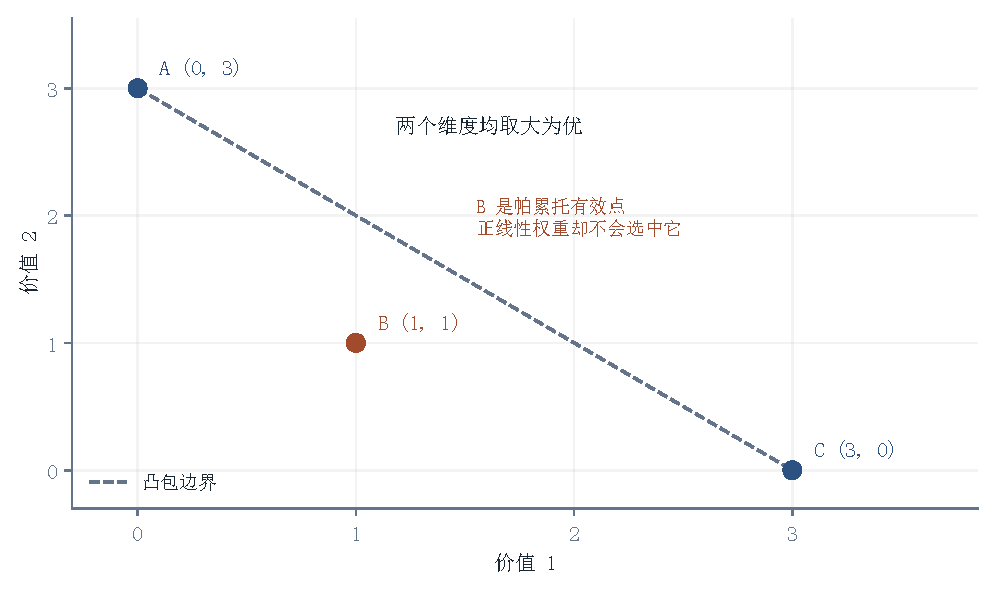
\includegraphics[width=\textwidth]{figures/unsupported-pareto.pdf}
\caption{可行集只有$A=(0,3)$、$B=(1,1)$与$C=(3,0)$，两个维度均取大为优。$B$不被其他点支配；但对$0\leq w\leq1$，$\max\{3w,3(1-w)\}\geq1.5>1$，线性加权不会选择$B$。}
\label{fig:mechanism-unsupported-pareto}
\end{figure}


\subhead{为什么这些位置长期报酬偏低}

如果这些位置承担着关键功能，一个自然的问题是它们为什么在很长一段时间里报酬不高。这个问题有两个答案，都是结构性的。第一是它们的价值难以度量。照护的成果是“没有出事”，教育的成果是“二十年后这个人过得如何”，事故调查的成果是“没有发生的灾难”。这些结果没有可比的计数，因此在以可量化指标为分配依据的体系里，它们的位置被系统性地压低。这是一个度量问题，不是价值问题。

第二是报酬形成的制度条件。某些经验与关系需要持续积累，供给扩张较慢；实际支付还取决于家庭资源、公共预算、雇佣规则与议价能力。私人服务可以扩大部分供给，也可能扩大获得服务的差距。功能的重要性、相对稀缺性与劳动者所得，必须分别观察。

\subhead{这个判断的边界}

验证、照护和长期塑造的相对稀缺性，需要与现有技术水平和制度配置共同判断。有些流程成本高，是因为缺少改造；另一些环节则承担了确有必要的功能。保留什么，取决于该功能如何被证明、能否用更低成本实现，以及取消后由谁承担损失。

这些功能也有身体消耗、责任压力、情绪劳动与机会成本。进入所需的长期投入，可能把缺乏时间和资源的人挡在外面。培养支持、公共支付、合理工作条件与进入机会，需要和技术工具一起改善，重要性才有机会转化为稳定供给与公平报酬。

如果价值最终沉淀在这些位置上，那么决定哪些问题值得投入的问题就变得更加关键。机器可以在给定的目标下高效搜索，但目标本身从哪里来，是接下来必须回答的问题。
